\documentclass[conference]{IEEEtran}
\IEEEoverridecommandlockouts
% The preceding line is only needed to identify funding in the first footnote. If that is unneeded, please comment it out.
\usepackage{cite}
\usepackage{amsmath,amssymb,amsfonts}
\usepackage{algorithmic}
\usepackage{graphicx}
\usepackage{textcomp}
\usepackage{xcolor}
\usepackage{tikz}
\usepackage[version=4]{mhchem}
\usepackage{booktabs}
\usepackage{multirow}
\usepackage{siunitx}
\usepackage{eurosym}
\usepackage{mhchem}
\usepackage{amssymb}
\usepackage{tikz}
\usepackage{pgfplots}
\usepackage{multirow}
\usepackage{graphicx}
\usepackage{hyperref}
\usepackage{eurosym}
\def\BibTeX{{\rm B\kern-.05em{\sc i\kern-.025em b}\kern-.08em
    T\kern-.1667em\lower.7ex\hbox{E}\kern-.125emX}}
\usepackage{url}

\newcommand{\red}[1]{\textcolor{red}{#1}}
\newcommand{\figspace}{\vspace{-0.5cm}}
\newcommand{\paragraphspace}{\vspace{-0.3cm}}
\begin{document}


\title{Synergy Among Flexible Demands: Forming a Coalition to Earn More from Reserve Market}

\author{Peter A.V. Gade\textsuperscript{*}\textsuperscript{\textdagger}, Trygve Skjøtskift\textsuperscript{\textdagger}, Henrik W. Bindner\textsuperscript{*}, Jalal Kazempour\textsuperscript{*} \\
    \textsuperscript{*}Department of Wind and Energy Systems, Technical University of Denmark, Kgs. Lyngby, Denmark \\
    \textsuperscript{\textdagger}IBM Client Innovation Center, Copenhagen, Denmark
    % <-this % stops a space
    \thanks{
        %Corresponding author. Tel.: +45 24263865. \\ 
        Email addresses: pega@dtu.dk (P.A.V. Gade), Trygve.Skjotskift@ibm.com (T. Skjøtskift), hwbi@dtu.dk (H.W. Bindner), jalal@dtu.dk (J. Kazempour).}% <-this % stops a space
    %    \thanks{Manuscript received April 19, 2021; revised August 16, 2021.} \\

    \vspace{-3mm}
}

% \footnote{Corresponding author. Tel.: +45 24263865. \\ Email addresses: pega@dtu.dk (P.A.V. Gade), Trygve.Skjotskift@ibm.com (T. Skjøtskift), hwbi@dtu.dk (H.W. Bindner), jalal@dtu.dk (J. Kazempour).}

% The paper headers
%\markboth{Journal of \LaTeX\ Class Files,~Vol.~14, No.~8, August~2021}%{Shell \MakeLowercase{\textit{et al.}}: A Sample Article Using IEEEtran.cls for IEEE Journals}

%\IEEEpubid{0000--0000/00\$00.00~\copyright~2021 IEEE}
% Remember, if you use this you must call \IEEEpubidadjcol in the second
% column for its text to clear the IEEEpubid mark.

\maketitle

% \tableofcontents

\IEEEaftertitletext{\vspace{-0.8\baselineskip}}
\maketitle
\thispagestyle{plain}
\pagestyle{plain}
\begin{abstract}
    % It has been well shown how demand-side flexibility can provide services to the power grid through an aggregator with no emissions. However, the aggregator still faces two, mostly unexplored, fundamental problems: 1) how many demand-side assets are needed in order to achieve a synergy effect? And 2) how are payments allocated to individual flexible demands downstream of the aggregator? This paper answers these two questions using simulations of uncertain assets to illustrate the synergy effect, and Shapley values are used as a payment allocation mechanism. As a use case, manual frequency restoration reserves (mFRR) are used as the ancillary service targeted by the aggregator with real prices from 2022.
    We address potential synergy among flexible demands and how they may earn more collectively than individually by forming a coalition and bidding to the reserve market.
    We consider frequency-supporting ancillary service markets, particularly the manual Frequency Restoration Reserve (mFRR) market.
    The coalition of flexible demands provides more reliable mFRR services, where in comparison to individual demands, is penalized less for their potential failure and is paid more for their successful activation. This synergy effect is quantified as a function of the number of homogeneous assets in the coalition. A subsequent payment allocation mechanism using Shapley values is proposed to distribute the total earnings of the coalition among demands, while incentivizing them to remain in the coalition. For our numerical study, we use real price data from the Danish mFRR market in 2022.
\end{abstract}

\begin{IEEEkeywords}
    Demand-side flexibility, synergy effect, manual frequency restoration reserve, Shapley values, payment allocation
\end{IEEEkeywords}

% TO BE DELETED
%\tableofcontents

\vspace{-2mm}
\section{Introduction}\label{sec:Introduction}
\subsection{Background}
It has been extensively addressed in the literature how the aggregation of flexible demands can provide frequency-supporting ancillary services to the power system \cite{biegel2014value}, \cite{macdonald2020demand}. By ancillary services, we refer to various forms of reserves, booked by the Transmission System Operator (TSO) in advance, to activate them in the operational stage, if necessary. The key for ancillary service provision by the aggregation of flexible demands is the availability of a \textit{baseline forecast} of total consumption. The TSO should approve in advance the process adopted by the aggregation of demands for their baseline forecast. This has been prescribed in the official documentation of the Danish TSO, Energinet, issued for the pre-qualification of demand-side resources for ancillary service provision \cite{energinet:prequalification}.

The aggregation of flexible demands is incentivized for at least two reasons: (\textit{i}) to meet the minimum bid size requirement, if existed, for ancillary service markets \cite{energinet:Systemydelser}, and (\textit{ii}) to unlock the potential \textit{synergy} among flexible demands. By synergy, we refer to operational circumstances under which the aggregation of flexible demands, compared to individual demands, may provide ancillary services with a higher level of reliability, i.e., a lower rate of delivery failure in the activation stage. By this, the whole aggregation is penalized less for their potential failure and paid more for their successful activation. We do not consider a case that, by aggregation, flexible demands may offer a larger volume of ancillary services. Hereafter, we refer to the aggregation of flexible demands as a \textit{coalition}, being operated by an \textit{aggregator}. Here, we consider that the aggregator represents the coalition, aiming to maximize the total profit of the coalition. The aggregator may charge flexible demands for its service, which is not part of this study.

Several private initiatives for the provision of demand-side flexibility via forming coalitions  are currently taking place in Denmark. For example, IBM is developing their \textit{Flex Platform}, aiming to aggregate and control heterogeneous assets in  commercial and industrial sectors. The aggregated flexibility is then shaped as flexibility services to be sold in various ancillary service markets running by the TSO, among which the market for manual Frequency Restoration Reserve (mFRR), also known as tertiary reserve, has usually the largest trading volume. The collected profit is supposed to be allocated among flexible demands in a fair manner. In addition, flexible demands might be further incentivized by being informed about their contribution to the CO$_{2}$ savings.

%\vspace{-3mm}
\subsection{Research questions and our contributions}
\vspace{-1mm}
Aggregation platforms such as the \textit{Flex Platform} of IBM face two fundamental questions: (\textit{i}) How many demand-side assets are needed to be aggregated in order to unlock the potential synergy,  resulting in sufficiently reliable ancillary services as prescribed by the TSO? and (\textit{ii}) How to allocate payments ex-post to individual flexible demands within the coalition?

We answer the first question by quantifying the synergy effect in terms of total earning of the coalition as a function of the number of assets within the coalition. For simplicity, we assume identical flexible assets, and limit our question to their number. The future work should extend the question by also considering the heterogeneity  of assets as a further degree of freedom. We show how individual assets are inherently unpredictable on their own, but comparatively more predictable within the coalition.

We then answer the second question by proposing Shapley values \cite{shapley1997value} as a mechanism to reward flexible demands for their contribution to the coalition. This provides desirable economic properties such as individual rationality and budget balance that incentivize flexible demands to stay in the coalition, as opposed to acting individually. We illustrate this payment mechanism  using a stylized example of five flexible demands, each with numerous assets, in a coalition, for which the aggregator bids in the mFRR market only. We conduct our simulations based on real price data of the Danish mFRR market from 2022.

%In this example, the first flexible provider only provides flexible capacity but no actual up-regulation. In this way, the penalty for doing so can be varied to assess the contribution of the flexible provider to the coalition.

%\IEEEpubidadjcol

%\subsection{Research questions}

%Thus, we aim to answer the following research questions:

%\begin{itemize}
%    \item How can the synergy effect be quantified for a portfolio of uncertain demand-side assets used for mFRR bidding?
%    \item How can payments be fairly allocated to flexible demands in an aggregator portfolio used for mFRR bidding such that each flexible provider is incentived to remain in the portfolio?
%\end{itemize}

\vspace{1mm}
\subsection{Status quo}
\vspace{-1mm}
Numerous studies in the literature explored important aspects of demand-side flexibility such as feasibility and controllability \cite{bondy2018redefining}, \cite{bondy2017performance}, \cite{bondy2016procedure}, \cite{bondy2014performance}, \cite{biegel2014integration}, \cite{AchievingControllabilityofElectricLoads}. However, an important aspect that has been largely overlooked is the potential synergy among demand-side assets, such as freezers, heat pumps, ventilation systems, etc.
%
Reference \cite{biegel2014value} investigates the value of flexible consumption but do not touch upon the synergy effect of a portfolio of assets, although it is mentioned that market barriers exist such as the minimum bidding size.
%
It has been shown in \cite{pedersen2014aggregation} how a portfolio of supermarkets can deliver a granular power response which is made possible by the number of supermarkets and their assets. Although it has not been explicitly mentioned, it refers to a form of synergy effect, because an aggregator requires a certain number of controllable assets to deliver a granular power response. However, the estimation and value of flexibility ex-ante is not tied together with any synergy effect. Note that  demand-side synergy is also known in other domains such as strategic and organizational diversification \cite{ye2012achieving}, but here we specifically address demand-side flexibility for ancillary services in power systems.

For the coalition of flexible demands, the baseline estimation is key, from which the aggregator estimates the flexible capacity, as prescribed by the Danish TSO \cite{energinet:prequalification}. Note that the coalition of flexible demands does not necessarily have an operational baseline schedule as a generation unit does \cite{gade2022ecosystem}.
%
In this work, we show how the baseline estimation becomes a more  straightforward task due to the synergy effect among assets within the coalition. In addition, it is important to estimate the baseline while being aware of potential counterfactual consumption when a flexible demand is activated. This problem has been studied extensively. Reference \cite{ziras2021baselines} explains why baselines are not necessarily suited for harnessing flexibility in the distribution grid, whereas \cite{capacity_limitation_services} instead shows how a mechanism based on capacity limitation services may work more successfully in practice. Nonetheless, for the TSO-level ancillary services aiming to instantaneously balance total production and total demand in the entire system, the baseline approach is generally adopted as a common practice. Some studies have proposed more innovative mechanisms as alternatives. For example,  \cite{muthirayan2019mechanism} proposes a mechanism by which the aggregator relies on self-reported baselines from individual flexible demands, removing the incentive to inflate baselines. In our setting, this is not straightforward to be implemented, since flexible demands have generally no capability or expertise to report their own baselines. Recall that flexible demands have their other primary business purposes, and prefer to not get involved in complicated mechanisms.
%Therefore, the aggregator has no incentive to inflate any of its flexible demands' baselines anyway. 
%In this work, we only rely on baseline estimation on the coalition level. Then Shapley values \cite{shapley1997value} are used as a mechanism to allocate payments to flexible demands within the portfolio as opposed to using baseline forecasts per flexible demand.


%\subsection{Our contributions and paper structure}

%As mentioned, we show two results related to the synergy effect of aggregating many individual demand-side assets with uncertain power consumption. The first is purely statistical and related to the estimation of reserve capacity from the aggregated portfolio versus the individual assets. The second result utilizes the synergy effect of individual \textit{coalitions} of flexibility providers within a portfolio to allocate payments using Shapley values. They provide a useful way for an aggregator to assess the performance of flexibility providers within its portfolio and directly allocate payments in an ex-post setting.


\vspace{0mm}
\subsection{Paper organization}
\vspace{-1mm}
The rest of the paper is organized as follows.
Section \ref{chapter2} introduces the proposed simulation setup. This includes an introduction to the mFRR services, an optimization model, and how Shapley values work as a payment mechanism in this context. Section \ref{chapter3} provides numerical results, illustrating the synergy among a number of assets and the corresponding payment allocation mechanism. Finally, Section \ref{chapter4} concludes the paper and outlines  potential directions for the future work.

\section{Simulation setup}
\label{chapter2}
%This section explains the simulation setup in detail. 

\subsection{mFRR services}\label{sec:mFRR}
%
Ancillary services including mFRR are exploited by the TSO to balance the power system such that at any instant the total production meets the total demand, maintaining the nominal power grid frequency (50 Hz in Europe). In Denmark, mFRR (as the tertiary reserve) is deployed after the activation of comparatively faster ancillary services when a frequency drop occurs --- mFRR is only used for up-regulation. The mFRR service providers are paid according to their (\textit{i}) capacity in terms of MW, and (\textit{ii}) up-regulation in terms of MWh, if activated. Often, the mFRR providers are not activated, so their upfront earning from the mFRR capacity availability constitutes a passive income. In our setup, we apply a penalty when the mFRR provider fails in the activation stage, i.e., the capacity does not match the actual up-regulation. For the coalition of flexible demands, this could happen  due to erroneous  flexible capacity estimation or unexpected failures when activating individual assets for up-regulation, e.g.,  because of violating the temperature thresholds of thermostatically controlled loads. %Bid prices are ignore for simplicity.
For further details about mFRR, see  \cite{energinet:prequalification}, \cite{energinet:Systemydelser}, and \cite{energinet:tender_conditions_reserves}.

\subsection{Optimization problem of the aggregator}
We use historical mFRR market prices, balancing market prices, and spot (day-ahead) market prices from DK1 bidding zone (western Denmark) in 2022 \cite{energinet:energidataservice}, denoted by $\lambda_{h}^{\text{mFRR}}$, $\lambda_{h}^{\text{b}}$, and $\lambda_{h}^{\text{s}}$, respectively,  for every hour $h$. The constant penalty price for the failure in the activation stage is denoted by $\lambda^{\text{p}}$. We assume a daily time horizon, and run the simulation for all days in 2022. For simplicity, we do not consider potential sources of uncertainty.

At the stage that the hourly baseline consumption forecasts $P^{\text{Base}}_{h}$ of the collation are given, the objective function of the aggregator is to maximize the total profit for the coalition, which can be mathematically formulated as
%
\begin{align}\label{eq:mFRRObjective}
     & \underset{p^{\text{mFRR}}_{h}, p^{\text{b},\uparrow}_{h}, p^{\text{b},\downarrow}_{h}, s_{h}}{\rm{maximize}} \ - \underbrace{\sum_{h=1}^{24} \lambda^{\text{s}}_{h}P^{\text{Base}}_{h}}_{\textrm{Energy cost}} + \underbrace{\sum_{h=1}^{24}\lambda_{h}^{\text{mFRR}} p^{\text{mFRR}}_{h}}_{\textrm{Reservation payment}}  \notag \\ & \quad \quad + \underbrace{\sum_{h=1}^{24}  \lambda_{h}^{\text{b}} p^{\text{b},\uparrow}_{h}}_{\textrm{Activation payment}} - \underbrace{\sum_{h=1}^{24}  \lambda_{h}^{\text{b}} p^{\text{b},\downarrow}_{h}}_{\textrm{Rebound cost}} - \underbrace{ \sum_{h=1}^{24}  \lambda^{\text{p}}s_{h}}_{\textrm{Penalty cost}}
\end{align}
where Greek and upper-case symbols represent parameters, while lower-case symbols are variables. The objective function includes the energy cost for purchasing baseline demands $P^{\text{Base}}_{h}$ at spot prices $\lambda^{\text{s}}_{h}$, the reservation payment by selling mFRR services $p^{\text{mFRR}}_{h}$ at mFRR market prices $\lambda_{h}^{\text{mFRR}}$, the activation payment for up-regulations (i.e., load reduction) $p^{\text{b},\uparrow}_{h}$ at balancing prices $\lambda_{h}^{\text{b}}$, the rebound cost by extra consumption $p^{\text{b},\downarrow}_{h}$ at balancing prices $\lambda_{h}^{\text{b}}$, and finally the penalty cost, incurred by the up-regulation not delivered $s_{h}$, penalized at the constant price $\lambda^{\text{p}}$. %Note that the first term (energy cost) is fixed and can be excluded from the objective function, however, we have included it for illustration purposes. 

%where the first term (energy cost) is fixed 
%Here, $p^{\text{mFRR}}_{h}$ is the hourly mFRR capacity of the aggregator portfolio, $p_{h}^{\text{b},\uparrow}$ is the real-time up-regulation, $p_{h}^{\text{b},\downarrow}$ is the rebound, $s_{h}$ is the energy not delivered, and $p^{\text{Base}}$ the normal operational baseline consumption.

For the sake of simplicity, we ignore the potential rebound effect of flexible demands by enforcing $p_{h}^{\text{b}, \downarrow} = 0, \ \forall{h}$. In addition, the energy cost is constant and can be removed from \eqref{eq:mFRRObjective}. Therefore, we rewrite the objective function as
%
\begin{align}\label{eq:mFRR_profit}
     & \underset{p^{\text{mFRR}}_{h}, p^{\text{b},\uparrow}_{h}, s_{h}}{\rm{maximize}} \ \underbrace{\sum_{h=1}^{24}\lambda_{h}^{\text{mFRR}} p^{\text{mFRR}}_{h}}_{\textrm{Reservation payment}} + \underbrace{\sum_{h=1}^{24}  \lambda_{h}^{\text{b}} p^{\text{b},\uparrow}_{h}}_{\textrm{Activation payment}} - \underbrace{ \sum_{h=1}^{24}  \lambda^{\text{p}}s_{h}}_{\textrm{Penalty cost}}
\end{align}

%The challenge for the aggregator in eq. (\ref{eq:mFRR_profit}) is therefore two-fold: 1) $p^{\text{mFRR}}_{h}$ must be estimated and 2) $s_{h}$ should be minimized.

In reality, there is a bidding process for both capacity and up-regulation, however, it is discarded for simplicity. Furthermore, we do not consider the control aspect of the coalition, i.e., the challenge of effectively following the required response within an hour of up-regulation.

%\subsection{Demand-side assets}

In \eqref{eq:mFRR_profit}, variables $p^{\text{mFRR}}_{h}$, $p^{\text{b},\uparrow}_{h}$, and $s_{h}$ correspond to the whole coalition. Each asset $i$ in the coalition has its own baseline for power consumption, $p_{h, i}$ $\forall{i} \in \mathcal{I}$, such that
%
\begin{subequations} \label{con}
    \begin{align}
        p^{\text{mFRR}}_{h}        & = \sum_{i} p^{\text{mFRR}}_{h, i}       \\
        p^{\text{b}, \uparrow}_{h} & = \sum_{i}p^{\text{b}, \uparrow}_{h, i} \\
        s_{h}                      & = \sum_{i} s_{h, i}.
    \end{align}
\end{subequations}
%
By this, the variable set of the optimization problem \eqref{eq:mFRR_profit}-\eqref{con} is extended to $p^{\text{mFRR}}_{h, i}$, $p^{\text{b}, \uparrow}_{h, i}$, $s_{h, i}$, $p^{\text{mFRR}}_{h}$, $p^{\text{b},\uparrow}_{h}$, and $s_{h}$.


%An asset is defined as any power consuming device\footnote{This including batteries in principle, but these are ignored here.} such as a heat pump, freezer, ventilation system, air condition unit, or boiler, etc. The aggregator can also have high-consuming assets such as a zinc galvanizing furnace, a swimming pool, waste-water centrifugation units, etc.

\subsection{Modeling individual baselines and quantifying the synergy}
For simplicity, we consider homogeneous assets that are supposed to consume 1 kW in one hour of the day, and do not consume any power during the rest of the day. An example for such an asset is a ventilation unit. We uniformly distribute assets with 1-hour 1-kW consumption over the day, such that the baseline forecast $p_{h, i}$ for asset $i$ in hour $h$ is defined as
%
\begin{align}\label{eq:uniform}
    p_{h,i} \thinspace = \begin{cases}
                             1 & \text{if} \quad h  \sim \mathcal{U}(1,24) \\
                             0 & \text{otherwise.}
                         \end{cases}
\end{align}

For an aggregator, it is therefore complex to estimate $p^{\text{mFRR}}_{h, i}$ individually, but as the number of assets increases, the consumption of the coalition converges to a predictable uniform consumption for all $h \in \{1, \hdots, 24 \}$, so $p^{\text{mFRR}}_{h}$ becomes more predictable. Here, the predictability simply means the prediction of the power consumption for the next day, for which more advanced methods can be used \cite{ziras2021baselines}.
This is a stylized example as most assets have some degree of predictability, but it is sufficient to show a  relevant problem for coalitions of small-scale, uncertain demand-side assets. 
%It is complex for the aggregator to estimate the reserve capacity of the coalition, but as the number of assets increases, it becomes more straightforward.
%Furthermore, our definition of an asset is valid for any type of asset, including thermostatically controlled loads. 
%For example, freezers might consume an extra, unexpected amount of energy due to food refills or other exogenous events. 
%In addition, the temperature thresholds might be violated which renders flexibility provision impossible. This situation is simulated as explained in the next section.

Given the profit definition as in \eqref{eq:mFRR_profit}, the synergy effect of the coalition can be quantified as
%
\begin{align}\label{eq:synergy_effect}
    \text{Synergy effect [\%]} = \frac{ \text{Coalition profit} }{ \sum_{i \in \mathbb{I}} \text{Asset \textit{i}'s profit} }
\end{align}
where the synergy effect is simply defined as the ratio between the coalition profit and the sum of individual asset profits. The difference between the two will be due to the activation payment and the penalty cost, as the reservation payments are the same.

\subsection{Shapley values as the payment mechanism}
%
The Shapley value is a well-known mechanism to allocate contributions in a cooperative game \cite{shapley1997value}. This notion fits perfectly with the concept of synergy effect in a coalition of flexible demands. By using Shapley values, we fairly allocate ex-post the total profit, expressed as in \eqref{eq:mFRR_profit}, collected by the aggregator, among flexible demands.


%Now, however, we consider a downstream problem of the aggregator, i.e., how much each flexible demand (with their assets) contributes to the whole portfolio \textit{ex-post} mFRR bidding. Hence, the aggregator has received a pot of money for the whole portfolio, i.e., eq. (\ref{eq:mFRR_profit}), and faces the problem of distributing it to the flexible demands.

Let $\mathcal{D}=\{1, \hdots, D \}$ denote the set of flexible demands $d$, where $|\mathcal{D}|$ is the number of flexible demands. Each demand may contain multiple assets, such that $|\mathcal{D}|$ demands altogether have assets $\mathcal{I}=\{1, \hdots, I \}$. Every asset is modeled using \eqref{eq:uniform}.
%
%$g$ are denoted $\mathcal{A}_{g,i} = \{1 \hdots N_g \}$. 
Inspired by \cite{shapley1997value}, the Shapley value $\phi_d$  for the flexible demand $d$, i.e., the payment allocated to that demand, is calculated by
%
\begin{align}\label{eq:shap}
    \phi_d & = \sum_{\mathcal{S} \subseteq \mathcal{D}, d \in \mathcal{S}} \frac{(|\mathcal{S}|-1)! \ (|\mathcal{D}|-|\mathcal{S}|)!}{|\mathcal{D}|!}\Big[v(\mathcal{S})-v(\mathcal{S} \backslash\{d\})\Big],
\end{align}
%
where $\mathcal{S}$ represents every possible non-empty subset of the coalition, $|\mathcal{S}|$ is the number of possible subsets,  and $v(\mathcal{S})$ is the value of the coalition subset $\mathcal{S}$, which is the corresponding profit formulated as in \eqref{eq:mFRR_profit}. Similarly, $v(\mathcal{S} \backslash\{d\})$ represents the value of coalition subset $\mathcal{S}$ excluding the flexible demand $d$ with its corresponding assets. The grand coalition is the one including all demands, whose value (profit) is given by $v(\mathcal{D}) = \sum_{d \in \mathcal{D}} \phi_{d}$.

%Here, $v$ is simply the profit in eq. (\ref{eq:mFRR_profit}). Thus, $v(\mathcal{S})$ represents the value of mFRR bidding for the portfolio of flexible demands given by the coalition $\mathcal{S}$. The value of the grand coalition, i.e., the whole portfolio is given by $v(\mathcal{G}) = \sum_{g \in \mathcal{G}} \phi_{g}$.

The Shapley value  in \eqref{eq:shap} can be thought of as the average marginal contribution of the flexible demand $d$ across all possible coalitions in $\mathcal{D}$. It can only be computed exactly for a relatively small number of flexible demands, as the number of  possible non-empty coalitions is equal to $2^{|\mathcal{D}|} - 1$. In this paper, we consider 5 demands, ending up in 31 possible coalitions. The Shapley values can be approximated when $|\mathcal{D}|$ grows \cite{castro2009polynomial}.
Note that the Shapley mechanism has desirable economic properties such as individual rationality (see Section \ref{chapter3}) and budget balance.

%Using Shapley values, the aggregator have a fair mechanism for the payment allocation. If one flexible demand has assets that marginally contribute with limited flexibility, it will be reflected in their Shapley value. For example, a flexible demand can have a relatively small portfolio of assets. More interestingly, a flexible demand can have many high-consuming assets that for some reason are not up-regulating when needed (as illustrated in Section \ref{section3}). Using Shapley values, the aggregator can ex-post determine how much such a flexible demand contributes with. Otherwise, that can be difficult to estimate for the aggregator due to the benefit of reserve payment versus risk of not being able to up-regulate.



\section{Results}\label{chapter3}

%In this section, we first show the assets being simulated and the flexible demands (groups) within the aggregated portfolio. Then results for the synergy effect is shown when the number of assets in the portfolio increases. Afterwards, we consider the payment allocation to flexible demands and investigate the impact of a flexible provider not delivering any up-regulation but only capacity.

%\subsection{Visualization of groups and assets}

We consider five flexible demands with 1000 assets in total. Each asset consumes 1 kW in one hour of the day, and nothing in the remaining hours. Figure \ref{fig:assets} shows the  consumption portfolio for a sample day, where 1000 assets, according to \eqref{eq:uniform}, are uniformly distributed among 24 hours. We consider 233 days with the same assets and ownership to five demands, however their consumption distribution over hours may differ.  

Figure x illustrates the mFRR market prices $\lambda^{\text{mFRR}}$ as well as balancing market prices $\lambda^{\text{b}}$ and spot (day-ahead) market prices $\lambda^{\text{s}}$ for 233 days, consistent with the real data in DK1 for 2022. The penalty price $\lambda^{\text{p}}$ is fixed to 0.1 DKK/kWh. 

%It is almost uniform and fairly predictable where each group is less predictable and each asset within each group even more so. The aggregated distribution approaches a uniform distribution as the number of assets increases.

\begin{figure}[!t]
    \centering
    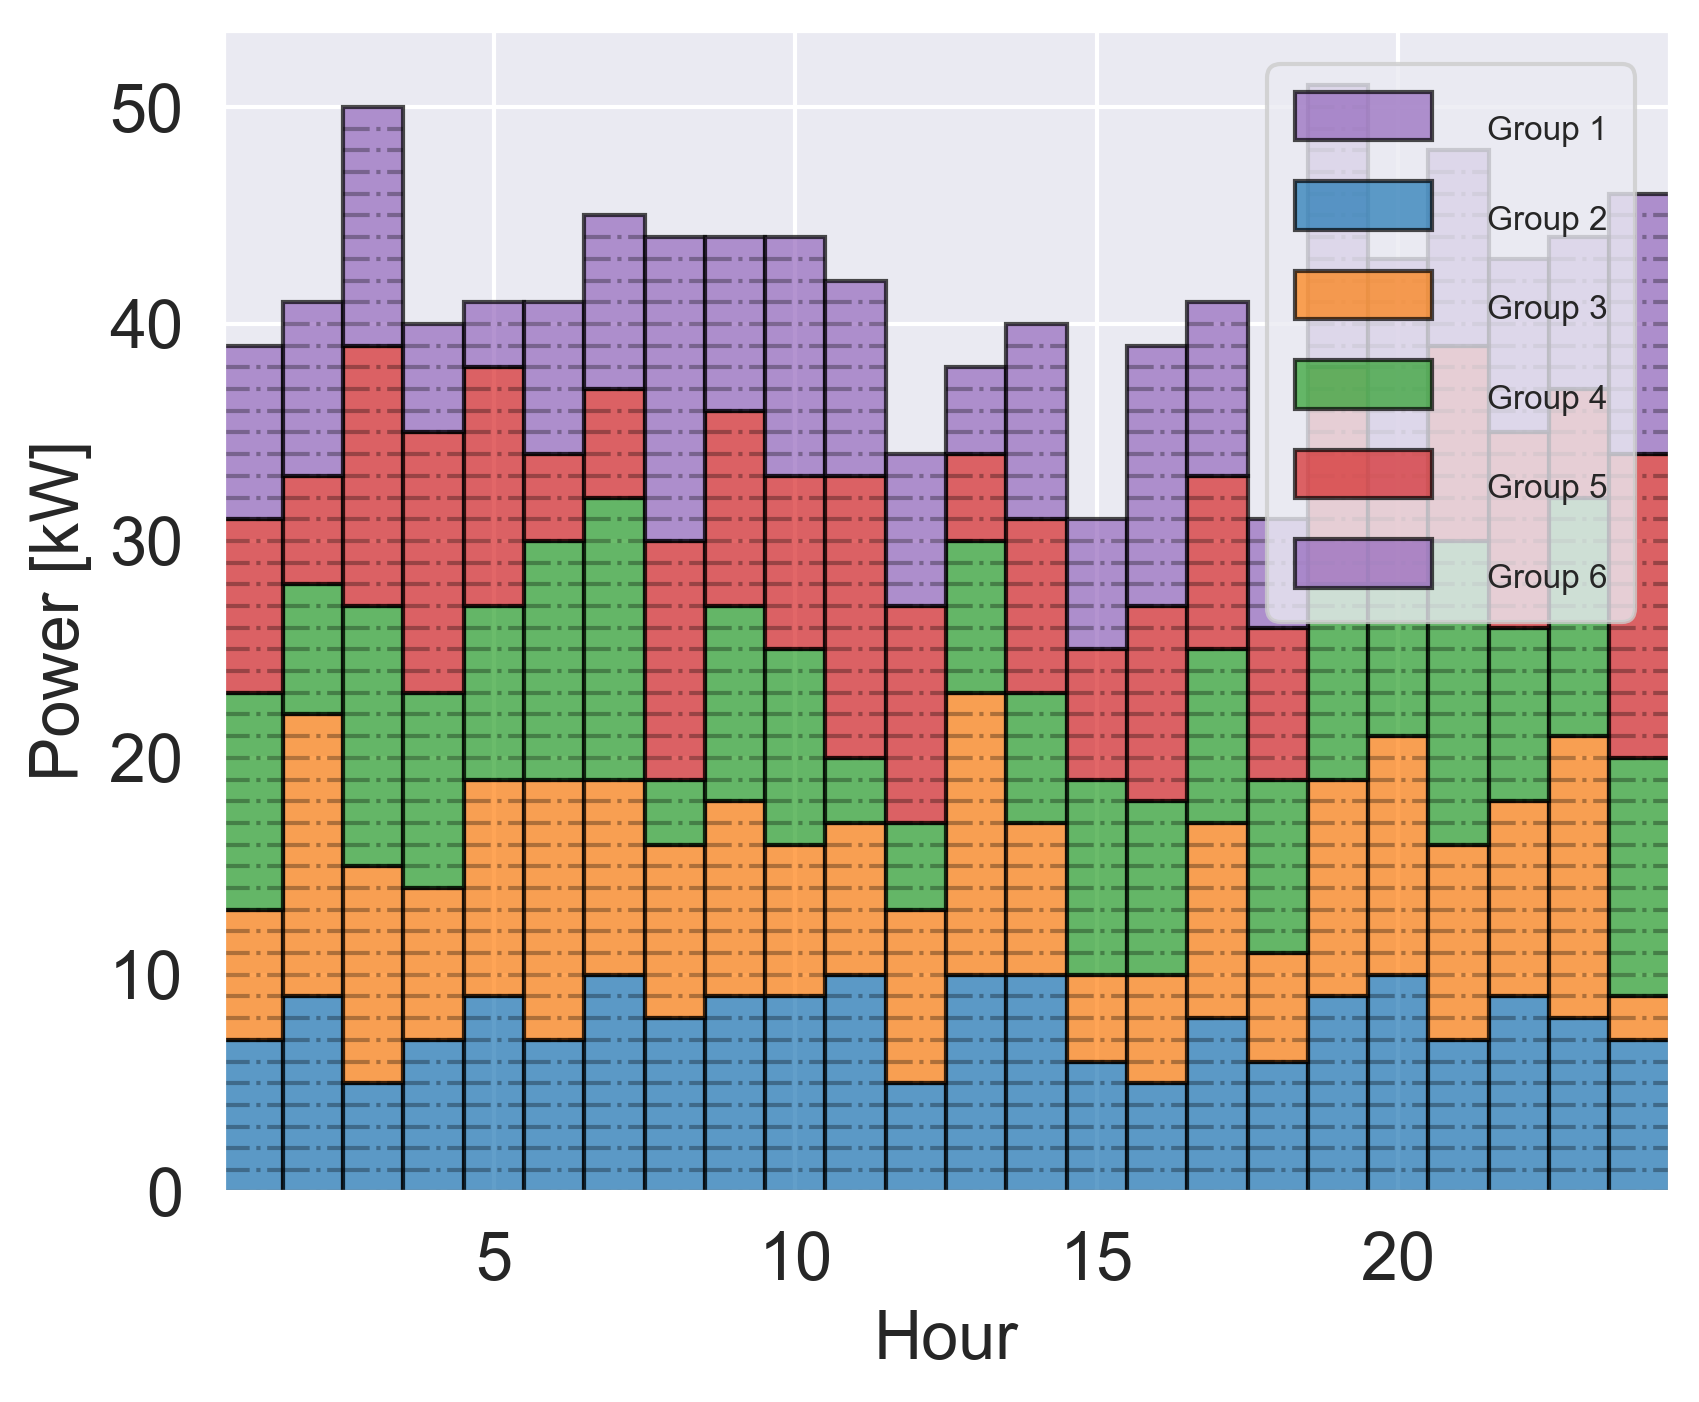
\includegraphics[width=\columnwidth]{figures/assets2.png}
    \caption{The consumption profile of a coalition with 1000 assets belonging to five flexible demands in a sample day. Each asset consumes 1 kW in one hour of the day.}
    \label{fig:assets}
\end{figure}

\subsection{Synergy effect of assets}

Figure \ref{fig:synergy_effect} shows the simulation of the synergy effect using eq. (\ref{eq:uniform}) and
eq. (\ref{eq:synergy_effect}) for up to 1000 assets. Even with such uncertain assets, it only takes around 150 of these before the synergy effect flattens. In reality, much fewer assets are then needed to estimate their reserve capacity due to many real-life assets having a more predictable consumption than here..

As discussed already, this of course ignores the synergy effect of controlling assets \textit{within} each hour to deliver a proper response. This probably requires a significant number of assets if all of them are ON/OFF controlled and if they are very heterogenous.

\begin{figure}[b]
    \centering
    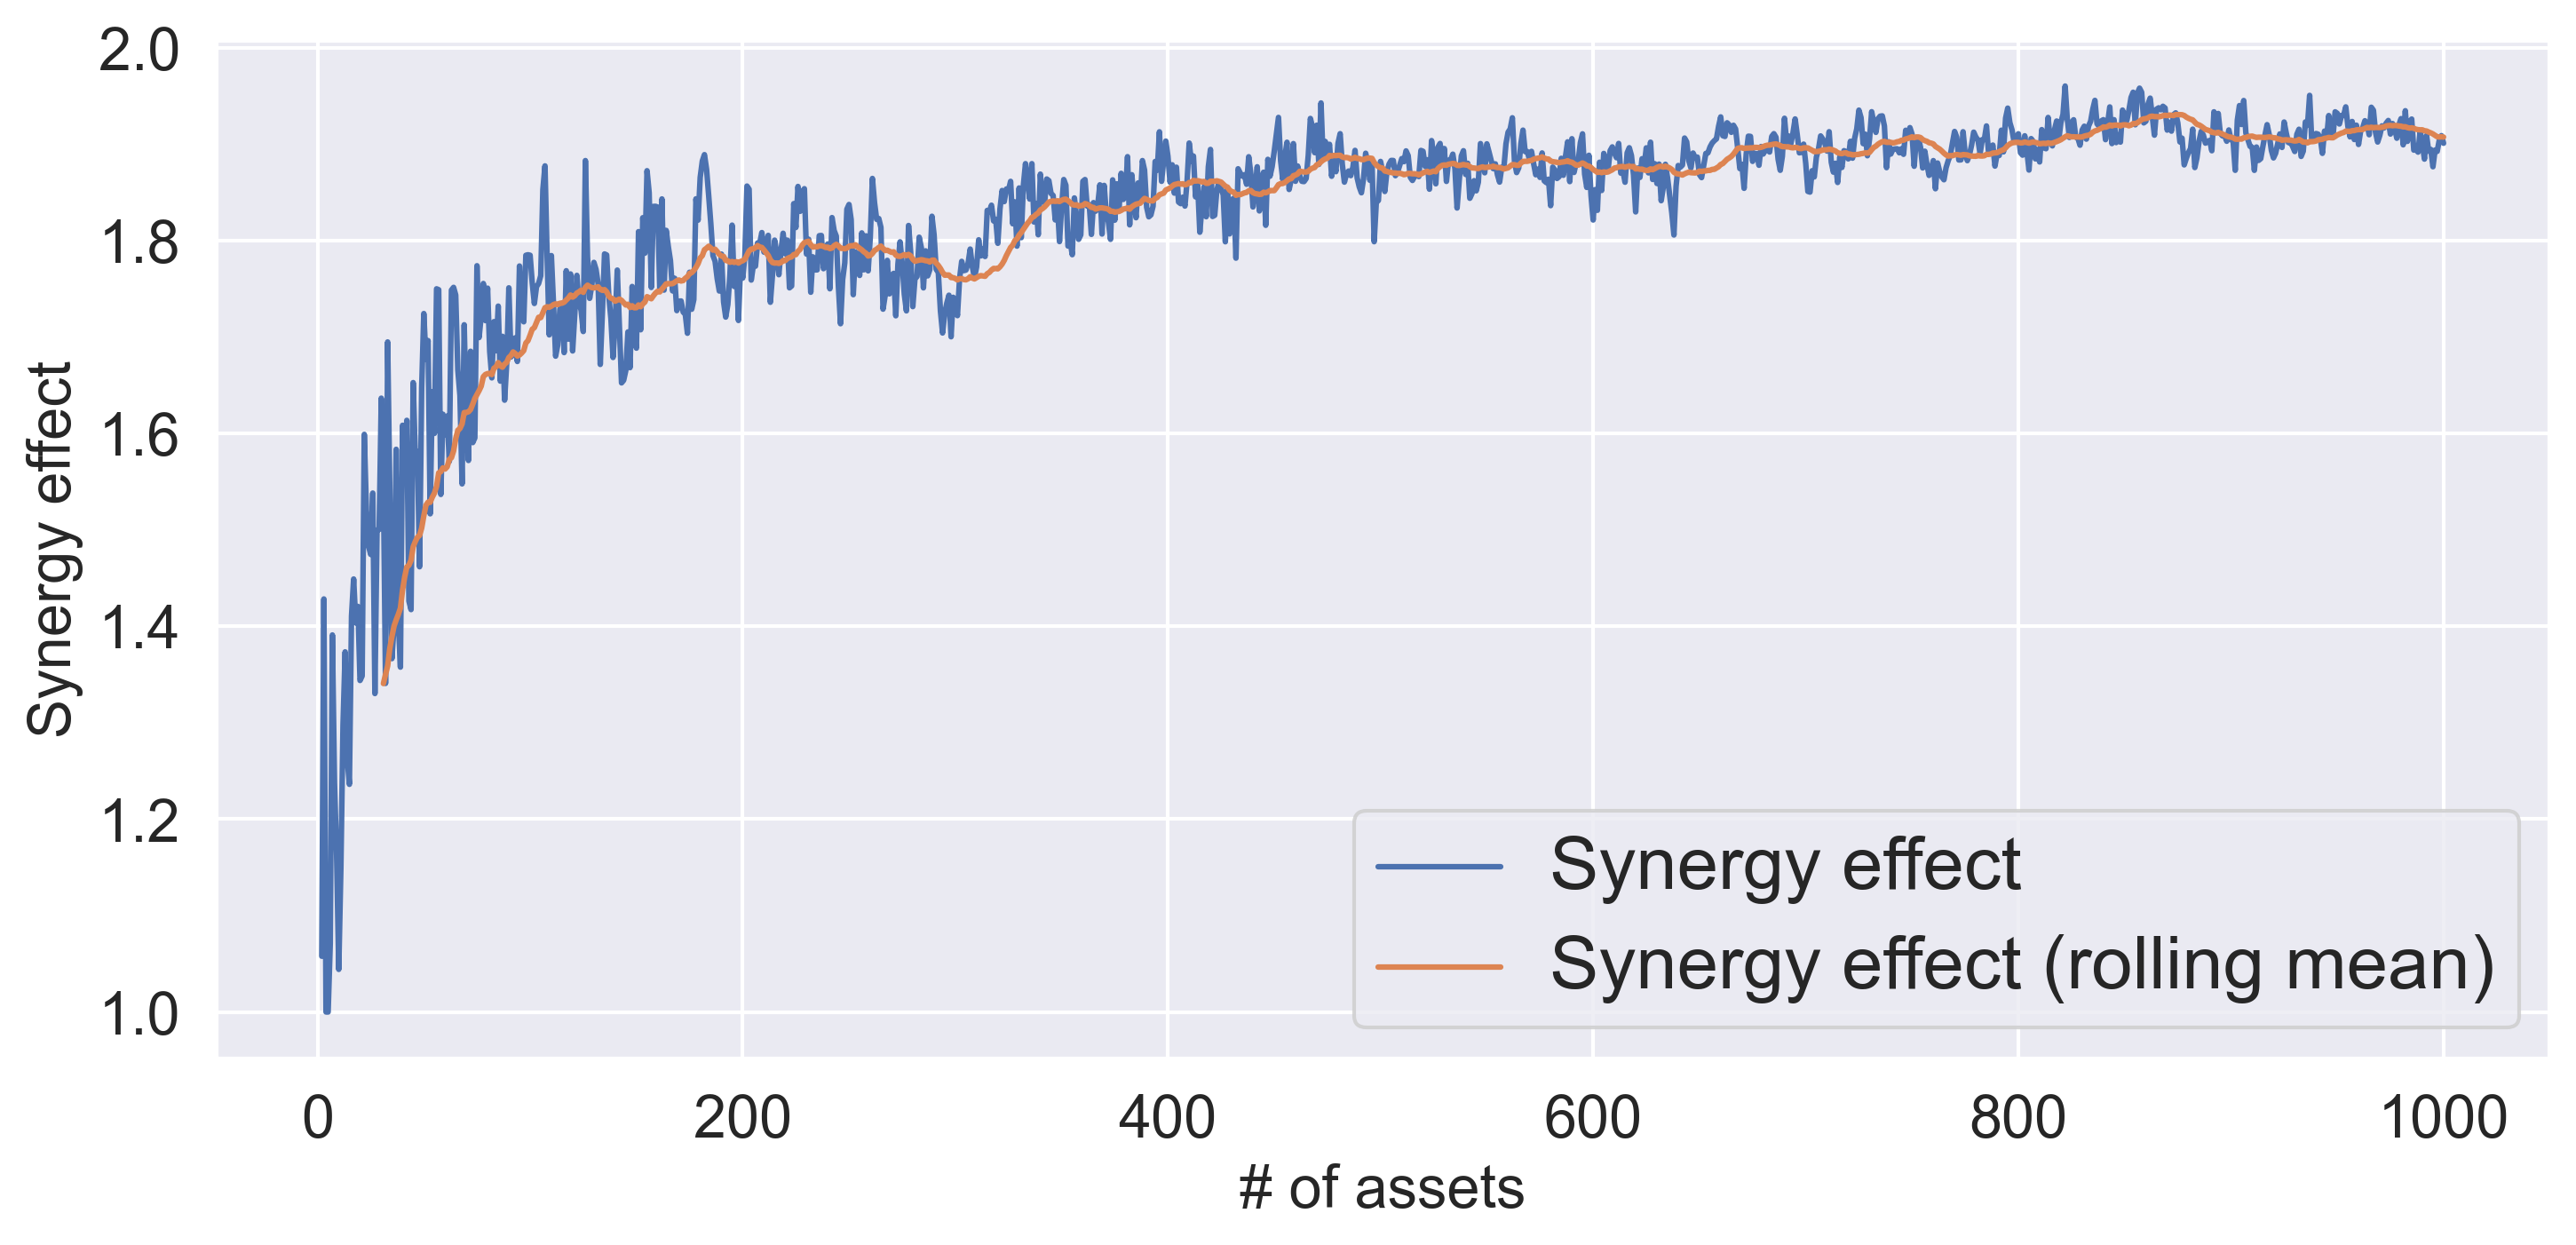
\includegraphics[width=\columnwidth]{figures/synergy_effect.png}
    \caption{Simulation of the impact on the synergy effect by increasing the number of assets. The rolling mean shows the average of the past 40 values.}
    \label{fig:synergy_effect}
\end{figure}

\subsection{Payment allocation}

Figure \ref{fig:shapley_values} shows the Shapley values for a simulation with $M = 5$, and where $g = 1$ has assets that never up-regulates and only contributes with their reserve capacity (which can never be utilized). The simulation is run for increasing values of the penalty parameter, $\lambda^{\text{p}}$.

Interestingly, it shows that $g_1$ actually contribute positively to the portfolio when $\lambda^{\text{p}} < 1.5$. This is simply explained by the price data and how often actual up-regulation is needed (which happens when $\lambda^{\text{b}} > \lambda^{\text{s}}$). If the power grid would need much more up-regulation, the cutoff for $\lambda^{\text{p}}$ would be lower.

The green and orange lines show individual rationality for coalition $G / \{1\}$. The orange line shows the total payment to $G / \{1\}$ when $g_1$ is included in the coalition, and the green line shows the total payment to $G / \{1\}$ when $g_1$ is \textit{not} included in the coalition. Intriguingly, it shows that $G / \{1\}$ benefits from having $g_1$ in the coalition even though $g_1$ gets negative payments. Hence, $G / \{1\}$ is better off with $g_1$ in the coalition.

Furthermore, $g_1$ also has individual rationality as seen by comparing the blue and red line. By being part of the grand coalition, $g_1$ gets paid more (or has to pay less back).

This readily illustrates individual rationality and the synergy effect of more flexible demands using Shapley values.


\begin{figure}[!t]
    \centering
    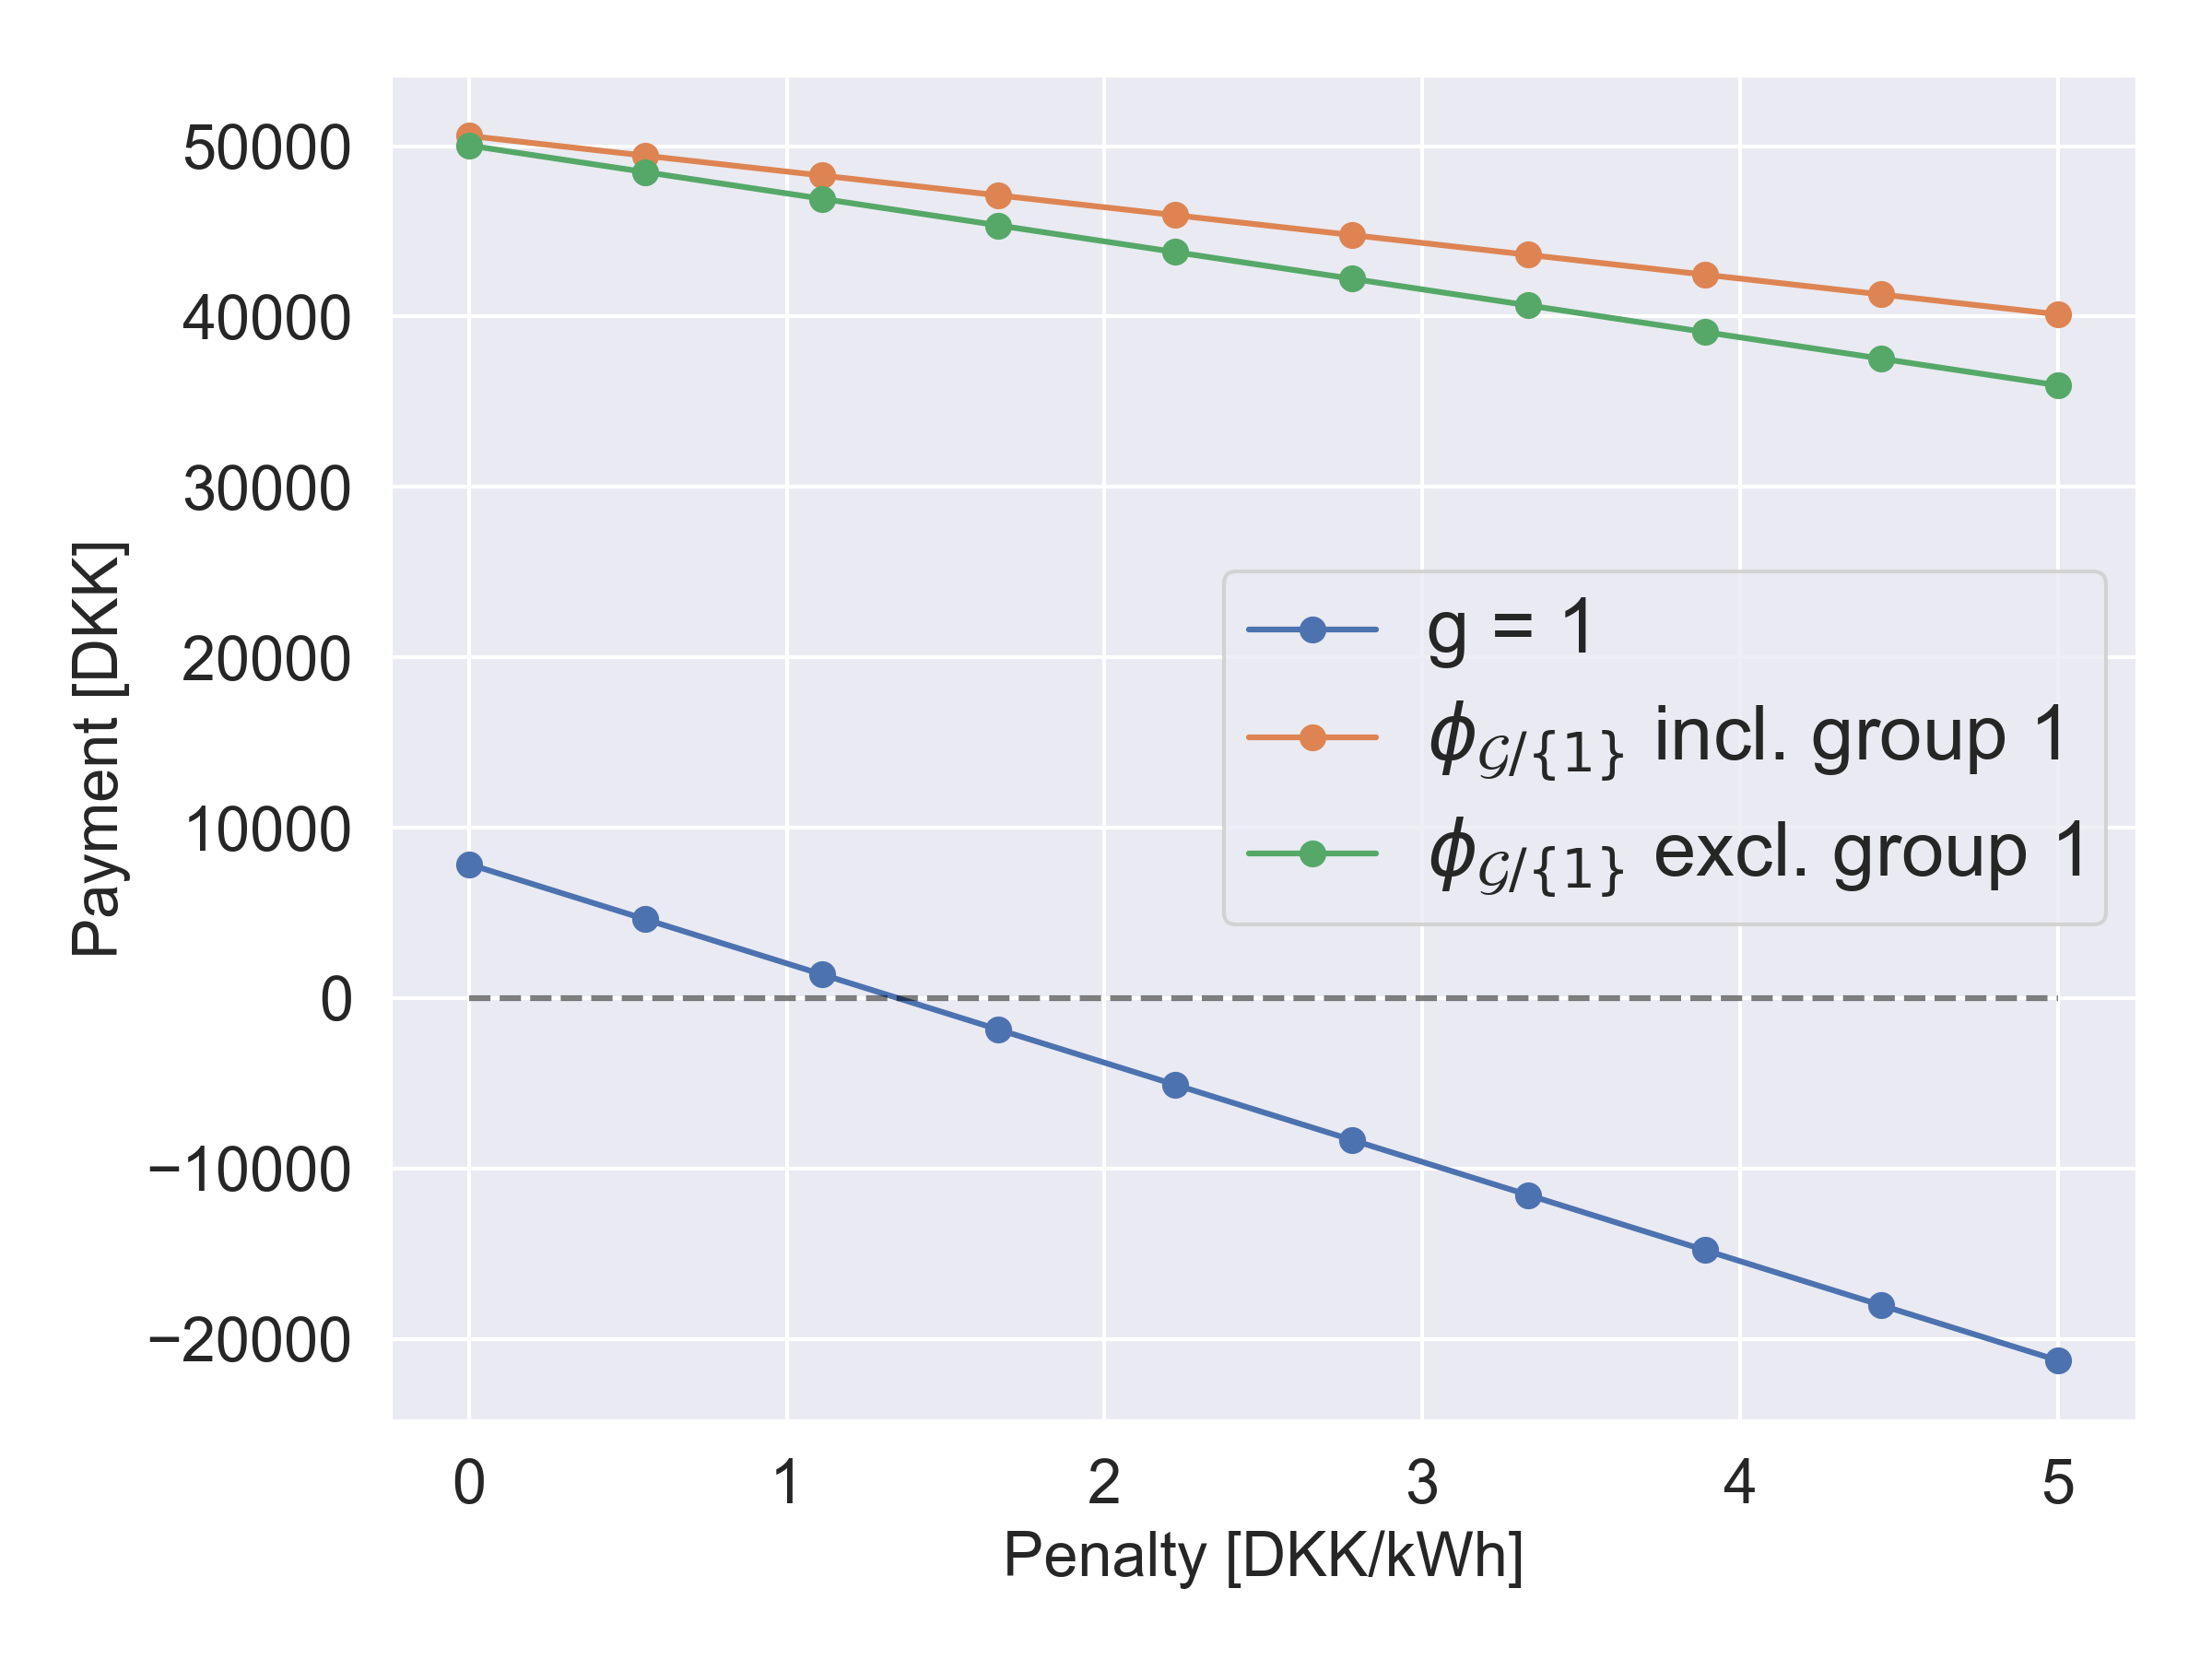
\includegraphics[width=\columnwidth]{figures/shapley_values.png}
    \caption{Simulation of the impact on Shapley values of the penalty price for not delivering promised capacity during up-regulation events. $g_1$ has assets with similar power consumption to $g_{2\hdots 5}$ but never up-regulates. The orange line shows payment to $G / \{1\}$ for the grand coalition, and the green line show payments to them if $g_1$ were not a part of the grand coalition. Likewise, the blue and red lines show payments to $g_1$ when participating in the grand coalition and on its own, respectively.}
    \label{fig:shapley_values}
\end{figure}


\section{Conclusion and Future Work}
\label{chapter4}

This paper demonstrated the synergy effect of a portfolio of uncertain demand-side assets in terms of numbers in the context of mFRR bidding. Furthermore, flexible demands within an aggregator portfolio, each with such uncertain assets, can be paid fairly using Shapley values. Our simulation showed that flexible demands have individual rationality and thus an incentive to participate in the portfolio as opposed to act on their own. Moreover, a flexible demand that never up-regulates was shown to contribute to the portfolio and get a positive payment when the penalty price for not delivering promised flexibility was low.

In this paper, two stylized examples of the same \textit{type} of assets were presented. However, one can also imagine a synergy effect across different types of assets so diversification of the portfolio provides a synergy effect. Hence, dissimilar assets can complement each other. One recent example of this could be Photovoltaic parks providing frequency services in conjunction with batteries or electrolysers increasing profits in synergy with a wind mill and/or batteries.

Moreover, as the number of flexible demands increase, approximate Shapley values must be used. It is interesting to explore how this impacts the fairness and distribution of payments.

\bibliographystyle{IEEEtran}
% \bibliography{tex/bibliography/Bibliography}
\bibliography{bibliography/Bibliography}


\vfill

\end{document}
